\documentclass[12pt, a4paper]{article}

\usepackage[utf8]{inputenc}
% Limit the page margin to only 1 inch.
\usepackage[margin=1in]{geometry}

%Imports biblatex package
\usepackage[
backend=biber,
style=alphabetic
]{biblatex}
\addbibresource{../../algs4e.bib}

% Enables the `align' environment.
\usepackage{amsmath}
% Provides useful environments, such as:
% - \begin{proof} ...\end{proof}
\usepackage{amsthm}
\usepackage[most]{tcolorbox}

\newtheorem*{proposition}{Proposition}

% Enables using \mathbb{}, for example \mathbb{N} for the set of natural numbers.
\usepackage{amssymb}

% Allows using letters in enumerate list environment. Use, for example:
%\begin{enumerate}[label=(\alph*)]
% ...
%\end{enumerate}
\usepackage[inline]{enumitem}

% Enable importing external graphic files and provides useful commannds, like \graphicspath{}
\usepackage{graphicx}
% Images are located in a directory called images in the current directory.
\graphicspath{{./images/}}

% Make links look better by default.
% See: https://tex.stackexchange.com/questions/823/remove-ugly-borders-around-clickable-cross-references-and-hyperlinks
\usepackage[hidelinks]{hyperref}
\usepackage{xcolor}
\hypersetup{
	colorlinks,
	linkcolor={red!50!black},
	citecolor={blue!50!black},
	urlcolor={blue!80!black}
}


% Code Listings. Source:
% https://stackoverflow.com/questions/3175105/inserting-code-in-this-latex-document-with-indentation
\usepackage{listings}
\usepackage{color}

\definecolor{dkgreen}{rgb}{0,0.6,0}
\definecolor{gray}{rgb}{0.5,0.5,0.5}
\definecolor{mauve}{rgb}{0.58,0,0.82}

\lstset{frame=tb,
	language=Java,
	aboveskip=3mm,
	belowskip=3mm,
	showstringspaces=false,
	columns=flexible,
	basicstyle={\small\ttfamily},
	numbers=none,
	numberstyle=\tiny\color{gray},
	keywordstyle=\color{blue},
	commentstyle=\color{dkgreen},
	stringstyle=\color{mauve},
	breaklines=true,
	breakatwhitespace=true,
	tabsize=3
}

\newcommand{\prob}{\text{P}}
%\newcommand{\complement}{\mathsf{c}}

% Define an environment called "ex" (for Exercise) so that I can do: \begin{ex}{1.5}...\end{ex}
\newenvironment{ex}[2][Exercise]
{\par\medskip\noindent \textbf{#1 #2.}}
{\medskip}

% Define a solution environment, similar to ex (exercise) environment.
\newenvironment{sol}[1][Solution]
{\par\medskip\noindent \textbf{#1.} }
{\medskip}

\begin{document}
	\noindent Sergio E. Garcia Tapia \hfill
	
	\noindent \emph{Algorithms} by Sedgewick and Wayne (4th edition) \cite{sedgewick_wayne}\hfill
	
	\noindent January 19, 2025\hfill 
	\section*{4.4: Shortest Paths}
	\begin{ex}{1}
		True or false: Adding a constant to every edge weight does not change the solution
		to the single-source shortest paths problem.
	\end{ex}
	\begin{sol}
		False. Consider the edge-weighted digraph on Figure~\ref{fig:ex-01a}. There is
		a negative cycle \texttt{3->4->5->3} reachable from \texttt{1}, so the single-source
		shortest paths problem has no solution when using \texttt{1} as the source,
		and any of vertices \texttt{3}, \texttt{4}, or \texttt{5} as the destination,
		according to \textbf{Proposition W}. However, if we add $0.2$ to all edge
		weights in the graph, then the negative cycle is eliminated, and now we have
		a solution.
		\begin{figure}
			\centering
			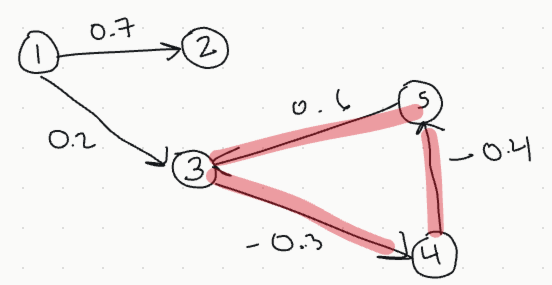
\includegraphics[width=0.3\textwidth]{exercise-01-a}
			\caption{Counterexample for statement in \textbf{Exercise 1}: Negative cycle}
			\label{fig:ex-01a}
		\end{figure}
		
		As another example, consider the graph in Figure~\ref{fig:ex-01-b}.
		If the graph has vertices \texttt{0}, \texttt{1}, and \texttt{2},
		with edge \texttt{0->1} with a weight of $0.1$, edge \texttt{1->2} with
		a weight of $0.2$, and edge \texttt{0->2} with a weight of $0.5$,
		then the single-source shortest-path problem with vertex \texttt{0}
		as the source has the solution \texttt{0->1->2}. But if we add
		$5$ to the weight of all edges, the solution is now \texttt{0->1} and
		\texttt{0->2}. In other words, adding a positive constant means that
		paths from the source to a destination that include more edges
		are affected more (they overall weight increment is more significant).
		\begin{figure}
			\centering
			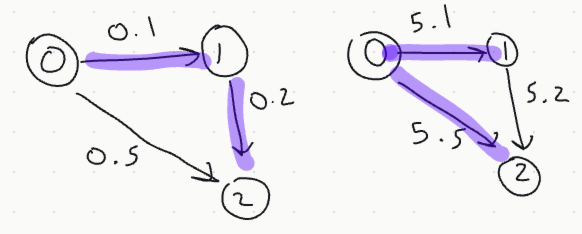
\includegraphics[width=0.3\textwidth]{exercise-01-b}
			\caption{Counterexample for statement in \textbf{Exercise 1}: Paths with more edges}
			\label{fig:ex-01-b}
		\end{figure}
	\end{sol}
	\begin{ex}{2}
		Provide implementations of the constructor \texttt{EdgeWeightedDigraph(In in)}
		and the method \texttt{toString()} for \texttt{EdgeWeightedDigraph}.
	\end{ex}
	\begin{sol}
		See \texttt{com.segarciat.algs4.ch4.sec4.ex02}.
	\end{sol}
	\begin{ex}{3}
		Develop an implementation of \texttt{EdgeWeightedDigraph} for dense graphs that
		uses an adjacency-matrix (two-dimensional array of weights) representation
		(see \textbf{Exercise 4.4.10}). Ignore parallel edges.
	\end{ex}
	\begin{sol}
		See \texttt{com.segarciat.algs4.ch4.sec4.ex03}.
	\end{sol}
	\begin{ex}{4}
		Draw the (unique) SPT for source \texttt{0} of the edge-weighted digraph obtained
		by deleting vertex \texttt{7} from \texttt{tinyEWD.txt} (see page 644), and give
		the parent-link representation of the SPT. Answer the question for the same digraph
		with all edges reversed.
	\end{ex}
	\begin{sol}
		After deleting vertex \texttt{7} and its associated edges, the remaining of
		\texttt{tinyEWD.txt} is:
		\begin{lstlisting}[language={}]
4 5  0.35
5 4  0.35
5 1  0.32
0 4  0.38
0 2  0.26
1 3  0.39
6 2  0.40
3 6  0.52
6 0  0.58
6 4  0.93
		\end{lstlisting}
		See Figure~\ref{fig:ex-04-a} for the SPT with \texttt{7} removed, and see
		Figure~\ref{fig:ex-04-b} for the SPT with \texttt{7} removed and edges reversed,
		both with \texttt{0} as source.
		\begin{figure}
			\centering
			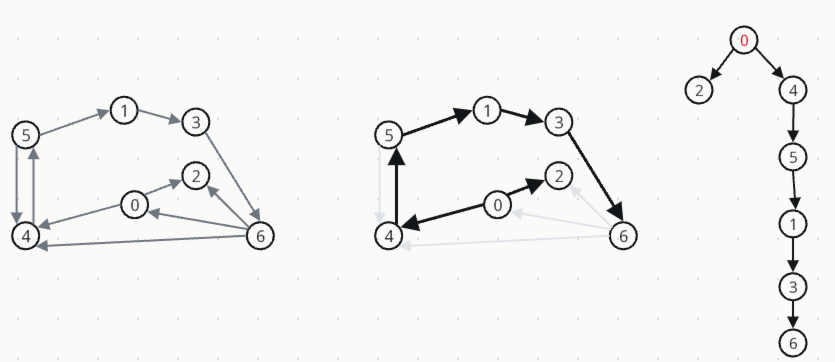
\includegraphics[width=0.6\textwidth]{exercise-04-a}
			\caption{SPT when parent link representation for the graph implied by
				\texttt{tinyEWD.txt} with \texttt{0} as source and vertex \texttt{7} removed.}
			\label{fig:ex-04-a}
		\end{figure}
		\begin{figure}
			\centering
			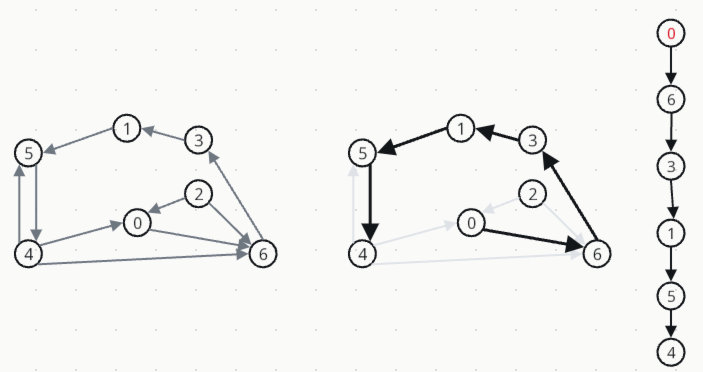
\includegraphics[width=0.6\textwidth]{exercise-04-b}
			\caption{SPT when parent link representation for the graph implied by
			\texttt{tinyEWD.txt} with \texttt{0} as source, vertex \texttt{7} removed,
			and all edges reversed.}
			\label{fig:ex-04-b}
		\end{figure}
	\end{sol}
	\begin{ex}{5}
		Change the direction of edge \texttt{0->2} in \texttt{tinyEWD.txt} (see page 644).
		Draw two different SPTs that are rooted at 2 for this modified edge-weighted
		digraph.
	\end{ex}
	\begin{sol}
		The full contents of \texttt{tinyEWD.txt} after reversal are:
		\begin{lstlisting}[language={}]
8
15
4 5  0.35
5 4  0.35
4 7  0.37
5 7  0.28
7 5  0.28
5 1  0.32
0 4  0.38
2 0  0.26
7 3  0.39
1 3  0.39
2 7  0.34
6 2  0.40
3 6  0.52
6 0  0.58
6 4  0.93
		\end{lstlisting}
		See Figure~\ref{fig:ex-05} for the resulting edge-weighted digraph and the
		shortest-path-tree. Note I was only able to find one SPT.
		\begin{figure}
			\centering
			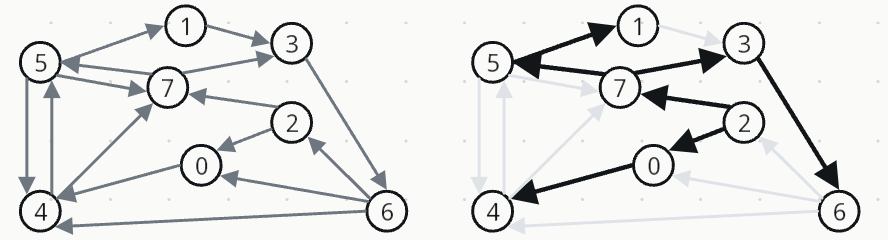
\includegraphics[width=0.6\textwidth]{exercise-05}
			\caption{Modified edge-weighted digraph after reversing edge \texttt{0->2}
			in \texttt{tinyEWD.txt}, and SPT rooted at 2.}
			\label{fig:ex-05}
		\end{figure}
	\end{sol}
	\begin{ex}{6}
		Give a trace that shows the process of computing the SPT of the digraph defined
		in \textbf{Exercise 4.4.5} with the eager version of Dijkstra's algorithm.
	\end{ex}
	\begin{sol}
		See Figure~\ref{fig:ex-06} for the full trace.
		\begin{figure}
			\centering
			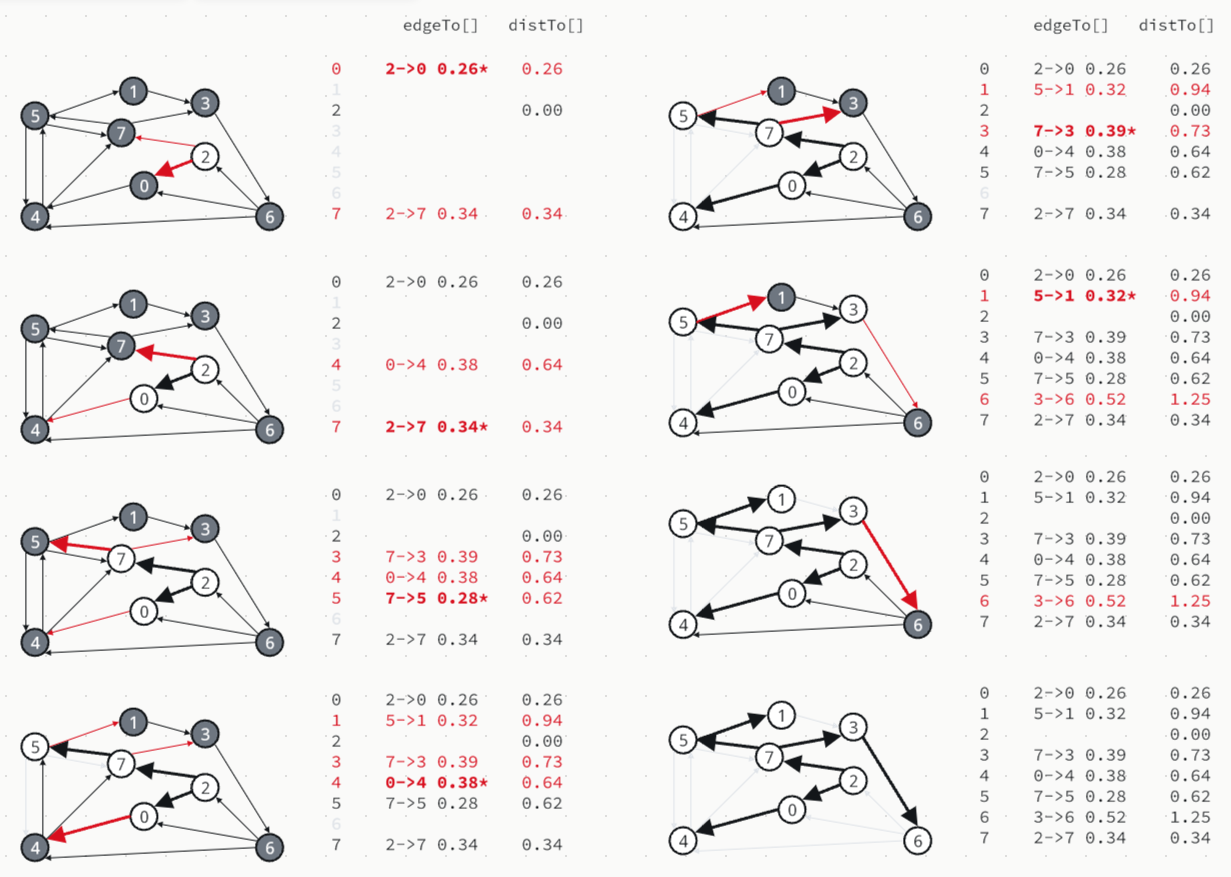
\includegraphics[width=0.9\textwidth]{exercise-06}
			\caption{Trace of the eager version of Dijsktra's algorithm to find the SPT
				rooted at 2 for the modified edge-weighted digraph after reversing edge
				\texttt{0->2} in \texttt{tinyEWD.txt}.}
			\label{fig:ex-06}
		\end{figure}
	\end{sol}
	\begin{ex}{7}
		Develop a version of \texttt{DijkstraSP} that supports a client method that returns
		a \emph{second}-shortest path from \texttt{s} to \texttt{t} in an edge-weighted digraph
		(and returns \texttt{null} if there is only one shortest path from \texttt{s} to \texttt{t}).
	\end{ex}
	\begin{sol}
		See \texttt{com.segarciat.algs4.ch4.sec4.ex07}.
	\end{sol}
	\begin{ex}{8}
		The \emph{diameter} of a digraph is the length of the maximum-length shortest
		path connecting two vertices. Write a \texttt{DijkstraSP} client that finds the
		diameter of a given \texttt{EdgeWeightedDigraph} that has nonnegative weights.
	\end{ex}
	\begin{sol}
		See \texttt{com.segarciat.algs4.ch4.sec4.ex08}.
	\end{sol}
	\begin{ex}{9}
		The table below, from an old published road map, purports to give the length
		of the shortest routes connecting the cities. It contains an error. Correct
		the table. Also, add a table that shows how to achieve the shortest routes.
		\begin{center}
			\begin{tabular}{c|cccc}
				{} & Providence & Westerly & New London & Norwich\\
				\hline
				Providence & - & 53 & 54 & 48\\
				\hline
				Westerly & 53 & - & 18 & 101\\
				\hline
				New London & 54 & 18 & - & 12\\
				\hline
				Norwich & 48 & 101 & 12 & -
			\end{tabular}
		\end{center}
	\end{ex}
	\begin{sol}
		The error is on the fourth row. It says that the shortest route from Norwich
		to Westerly is 101 units. But it also says that the shortest route from
		Norwich to New London is 12 units, and the shortest route from New London
		to Westerly is 18 units, which would imply that the shortest route from
		Norwich to Westerly is 30 units, not 101. To correct the table, I created
		a \texttt{DijkstraSP} client, from which I created the following table:
		\begin{center}
			\begin{tabular}{c|cccc}
				{} & Providence & Westerly & New London & Norwich\\
				\hline
				Providence & - & 53 & 54 & 48\\
				\hline
				Westerly & 53 & - & 18 & 30\\
				\hline
				New London & 54 & 18 & - & 12\\
				\hline
				Norwich & 48 & 30 & 12 & -
			\end{tabular}
		\end{center}
		See \texttt{com.segarciat.algs4.ch4.sec4.ex09}.
	\end{sol}
	\begin{ex}{10}
		Consider the edges in the digraph defined in \textbf{Exercise 4.4.4} to be undirected
		edges such that each edge corresponds to equal-weight edges in both directions
		in the edge-weighted digraph. Answer \textbf{Exercise 4.4.6} for this corresponding
		edge-weighted digraph.
	\end{ex}
	\begin{ex}{11}
		Use the memory-cost model of \textbf{Section 1.4} to determine the amount of memory
		used by \texttt{EdgeWeightedDigraph} to represent a graph with $V$ vertices and
		$E$ edges.
	\end{ex}
	\begin{sol}
		\texttt{EdgeWeightedDigraph} requires 16 bytes of object overhead, 4 bytes
		for its \texttt{int V} field, 4 bytes for its \texttt{int E} field,
		8 bytes for its reference to the array field \texttt{Bag<DirectedEdge>[] adj},
		and 24 bytes for the cost of the array itself, which makes for a flat cost of 56 bytes.
		The array \texttt{adj} has $8V$ references to \texttt{Bag<DirectedEdge>}, one for each
		adjacency list. Each \texttt{Bag<DirectedEdge>} requires 16 bytes of object
		overhead, 4 bytes for its \texttt{int size} field, 8 bytes for its \texttt{Node first}
		field, and 4 bytes of padding, for a cost of 32 bytes; since there are $V$ of them,
		this amounts to $8V+32V=40V$ bytes. Now, for each \texttt{DirectedEdge}, we have
		a \texttt{Node} object that has a $40$ byte cost. Meanwhile, the \texttt{DirectedEdge}
		itself requires 16 bytes of object overhead, 4 bytes for its \texttt{int v} field,
		4 bytes for its \texttt{int w} field, and 8 bytes for its \texttt{double weight}
		field, amounting to $32$ bytes. Since there are $E$ of them, together with the cost
		of their corresponding \texttt{Node} wrapper nodes, this amounts to $72$ bytes.
		
		The overall cost is $56+40V+72E$ bytes.
	\end{sol}
	\begin{ex}{12}
		Adapt the \texttt{DirectedCycle} and \texttt{Topological} classes from \textbf{Section 4.2}
		to use the \texttt{EdgeWeightedDigraph} and \texttt{DirectedEdge} APIs of this
		section, thus implementing \texttt{EdgeWeightedDirectedCycle} and \texttt{Topological}
		classes.
	\end{ex}
	\begin{sol}
		See \texttt{com.segarciat.algs4.ch4.sec4.ex12}.
	\end{sol}
	\begin{ex}{14}
		Show the paths that would be discovered by the two strawman approaches described
		on page 668 for the example \texttt{tinyEWDn.txt} shown on that page.
	\end{ex}
	\begin{sol}
		The file \texttt{tinyEWDn.txt} has the contents:
		\begin{lstlisting}[language={}]
8
15
4->5  0.35
5->4  0.35
4->7  0.37
5->7  0.28
7->5  0.28
5->1  0.32
0->4  0.38
10->2  0.26
7->3  0.39
1->3  0.29
2->7  0.34
6->2 -1.20
3->6  0.52
6->0 -1.40
6->4 -1.25
		\end{lstlisting}
		The actual SPT from \texttt{0} is depicted in Figure~\ref{fig:ex-14-actual}
		\begin{figure}
			\centering
			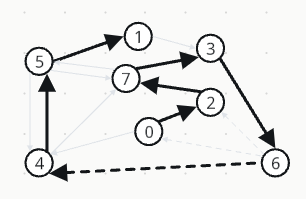
\includegraphics[width=0.4\textwidth]{exercise-14-actual-result}
			\caption{Actual SPT from \texttt{0} for \texttt{tinyEDWn.txt} (negative-weighted edges).}
			\label{fig:ex-14-actual}
		\end{figure}
		Strawman I suggests adding the absolute value of the most negative weight to
		all edges. In this case, that value is $|-1.40|=1.40$:
		\begin{lstlisting}[language={}]
8
15
4->5  1.75
5->4  1.75
4->7  1.77
5->7  1.68
7->5  1.68
5->1  1.72
0->4  1.78
0->2  1.66
7->3  1.79
1->3  1.69
2->7  1.74
6->2  0.20
3->6  1.92
6->0  0.00
6->4  0.15
		\end{lstlisting}
		See Figure~\ref{fig:ex-14-s1}.
		\begin{figure}
			\centering
			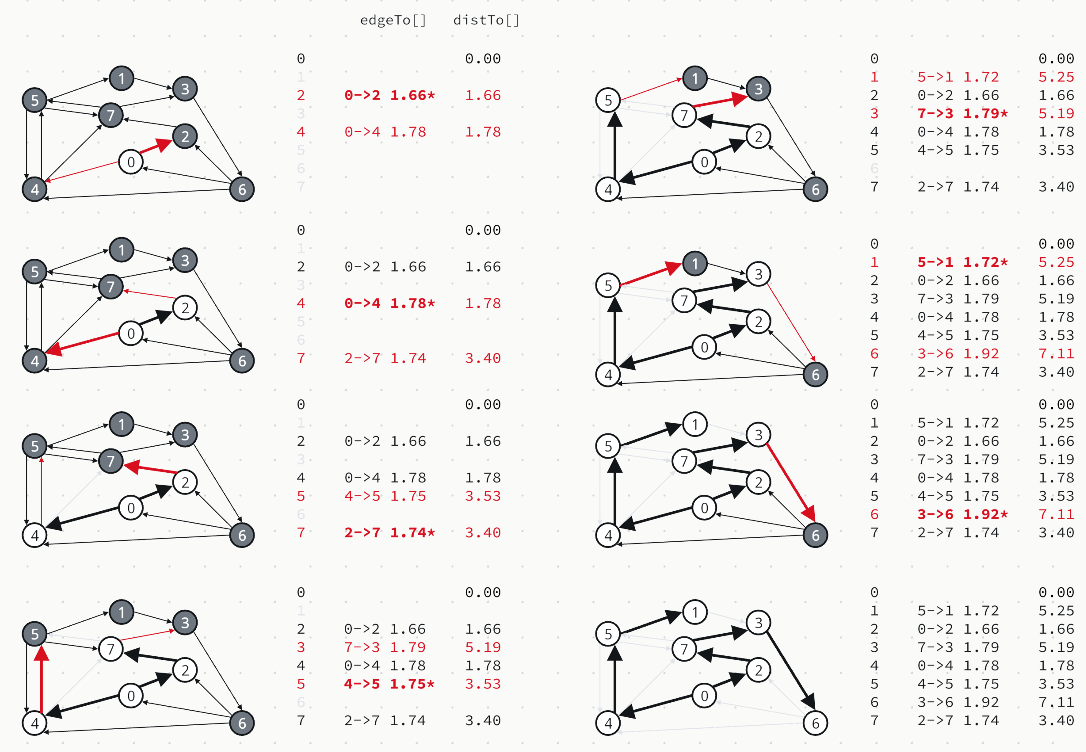
\includegraphics[width=0.9\textwidth]{exercise-14-strawman-1-trace}
			\caption{Strawman 1 for \texttt{tinyEWDn.txt} for an SPT from 0, using Dijkstra's algorithm.}
			\label{fig:ex-14-s1}.
		\end{figure}
	\end{sol}
	\begin{ex}{15}
		What happens to Bellman-Ford if there is a negative cycle on the path from
		\texttt{s} to \texttt{v} and then you call \texttt{pathTo(v)}?
	\end{ex}
	\begin{sol}
		It would result in an out of memory error because the program would fall into
		an infinite loop. The problem is that when a negative cycle is encountered,
		the \texttt{edgeTo} entry for the first vertex in the cycle is overwritten
		by the last vertex by the last edge in the cycle. Therefore, when the
		parent-tree representation climbs back up, it will not go further than
		the first edge in the cycle, and will continue to enqueue the same cycle
		edges.
	\end{sol}
	\begin{ex}{16}
		Suppose that we convert an \texttt{EdgeWeightedGraph} into an \texttt{EdgeWeightedDigraph}
		by creating two \texttt{DirectedEdge} objects in the \texttt{EdgeWeightedDigraph}
		(one in each direction) for each \texttt{Edge} in the \texttt{EdgeWeightedGraph}
		(as described for Dijkstra's algorithm in the Q\&A on page 684) and then use the
		Bellman-Ford algorithm. Explain why this approach fails spectacularly.
	\end{ex}
	\begin{sol}
		If a negative edge is present, then that edge is duplicated (once in each direction),
		creating a negative cycle. Since the digraph corresponds to the undirected
		graph, it is strongly connected, and hence the negative cycle is in the path
		to \emph{every} vertex from \emph{any} vertex.
	\end{sol}
	\begin{ex}{17}
		What happens if you allow a vertex to be enqueued more than once in the same pass
		in the Bellman-Ford algorithm?
	\end{ex}
	\begin{sol}
		According to Sedgewick and Wayne, the running time can go exponential.
	\end{sol}
	\begin{ex}{18}
		Write a \texttt{CPM} client that prints all critical paths.
	\end{ex}
	\begin{sol}
		See \texttt{com.segarciat.algs4.ch4.sec4.ex18}.
	\end{sol}
	\begin{ex}{19}
		Find the lowest-weight cycle (best arbitrage opportunity) in the example shown in
		the text.
	\end{ex}
	\begin{ex}{20}
		Find a currency-conversion table online or in a newspaper. Use it to build an
		arbitrage table. \emph{Note}: Avoid tables that are derived (calculated) from
		a few values and that therefore do not give sufficiently accurate conversion
		information to be interesting. \emph{Extra credit}: Make a killing in the
		money-exchange market!
	\end{ex}
	\begin{ex}{21}
		Show, in the style of the trace in the text, the process of computing the SPT with
		the Bellman-Ford algorithm for the edge-weighted digraph of \textbf{Exercise 4.4.5}.
	\end{ex}
	\begin{sol}
		See Figure~\ref{fig:ex-21-bf}.
		\begin{figure}
			\centering
			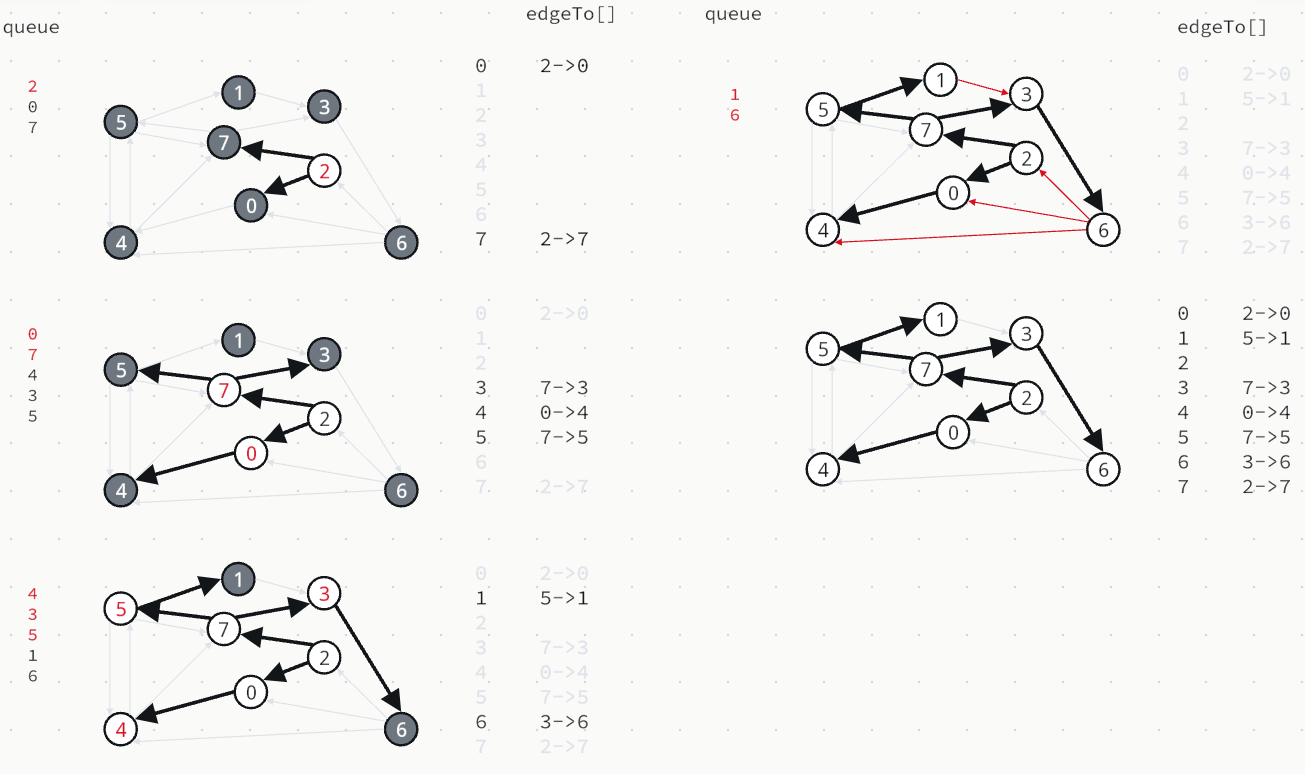
\includegraphics[width=0.4\textwidth]{exercise-21}
			\caption{Trace of Bellman-Ford algorithm for \textbf{Exercise 21}.}
			\label{fig:ex-21-bf}
		\end{figure}
	\end{sol}
	\pagebreak
	\printbibliography
\end{document}